%!TEX root = ../MasterThesis.tex

\section{Evaluation of existing design approaches}
\label{sec:system_approaches}

When trying to solve issues of information integration between organizations there are already existing solutions, that have to be examined whether they might fit the \gls{E-commerce} fraud investigation scenario or not. This section looks into common existing approaches to collect and integrate information between \gls{IT} systems.

\subsection{\gls{ETL} processes}
\label{subsec:etl_process}

To begin with, retrieving, transforming and combining data from multiple dispersed data sources is not a completely new problem, and is actually part of ``Extract-Transform-Load'' (\gls{ETL}) processes \emph{within} an organization. The basic idea is very much the same as in the concept shown in this thesis; namely to get as much information as possible from the various databases that are in use within a company, harmonize (aka transform) the data from each of them into a shared data model, and use the cleaned up and combined information repository for doing advanced business analytics and predictions later. Data within an organization is created and maintained by different business-related software tools. Each of these will usually store the information into their own database using a vendor-specific database schema. Other business-relevant information might be stored in structured files, sometimes using a proprietary format such as Microsoft Excel. Each of these data sources have to be accessed, the valuable information have to be extracted and mapped against each other, before the analysis of it can begin in a separate data store that holds the combined data set. The whole process is visualized in Figure~\ref{fig:images_etl_process}. \@

\begin{figure}[H]
  \centering
  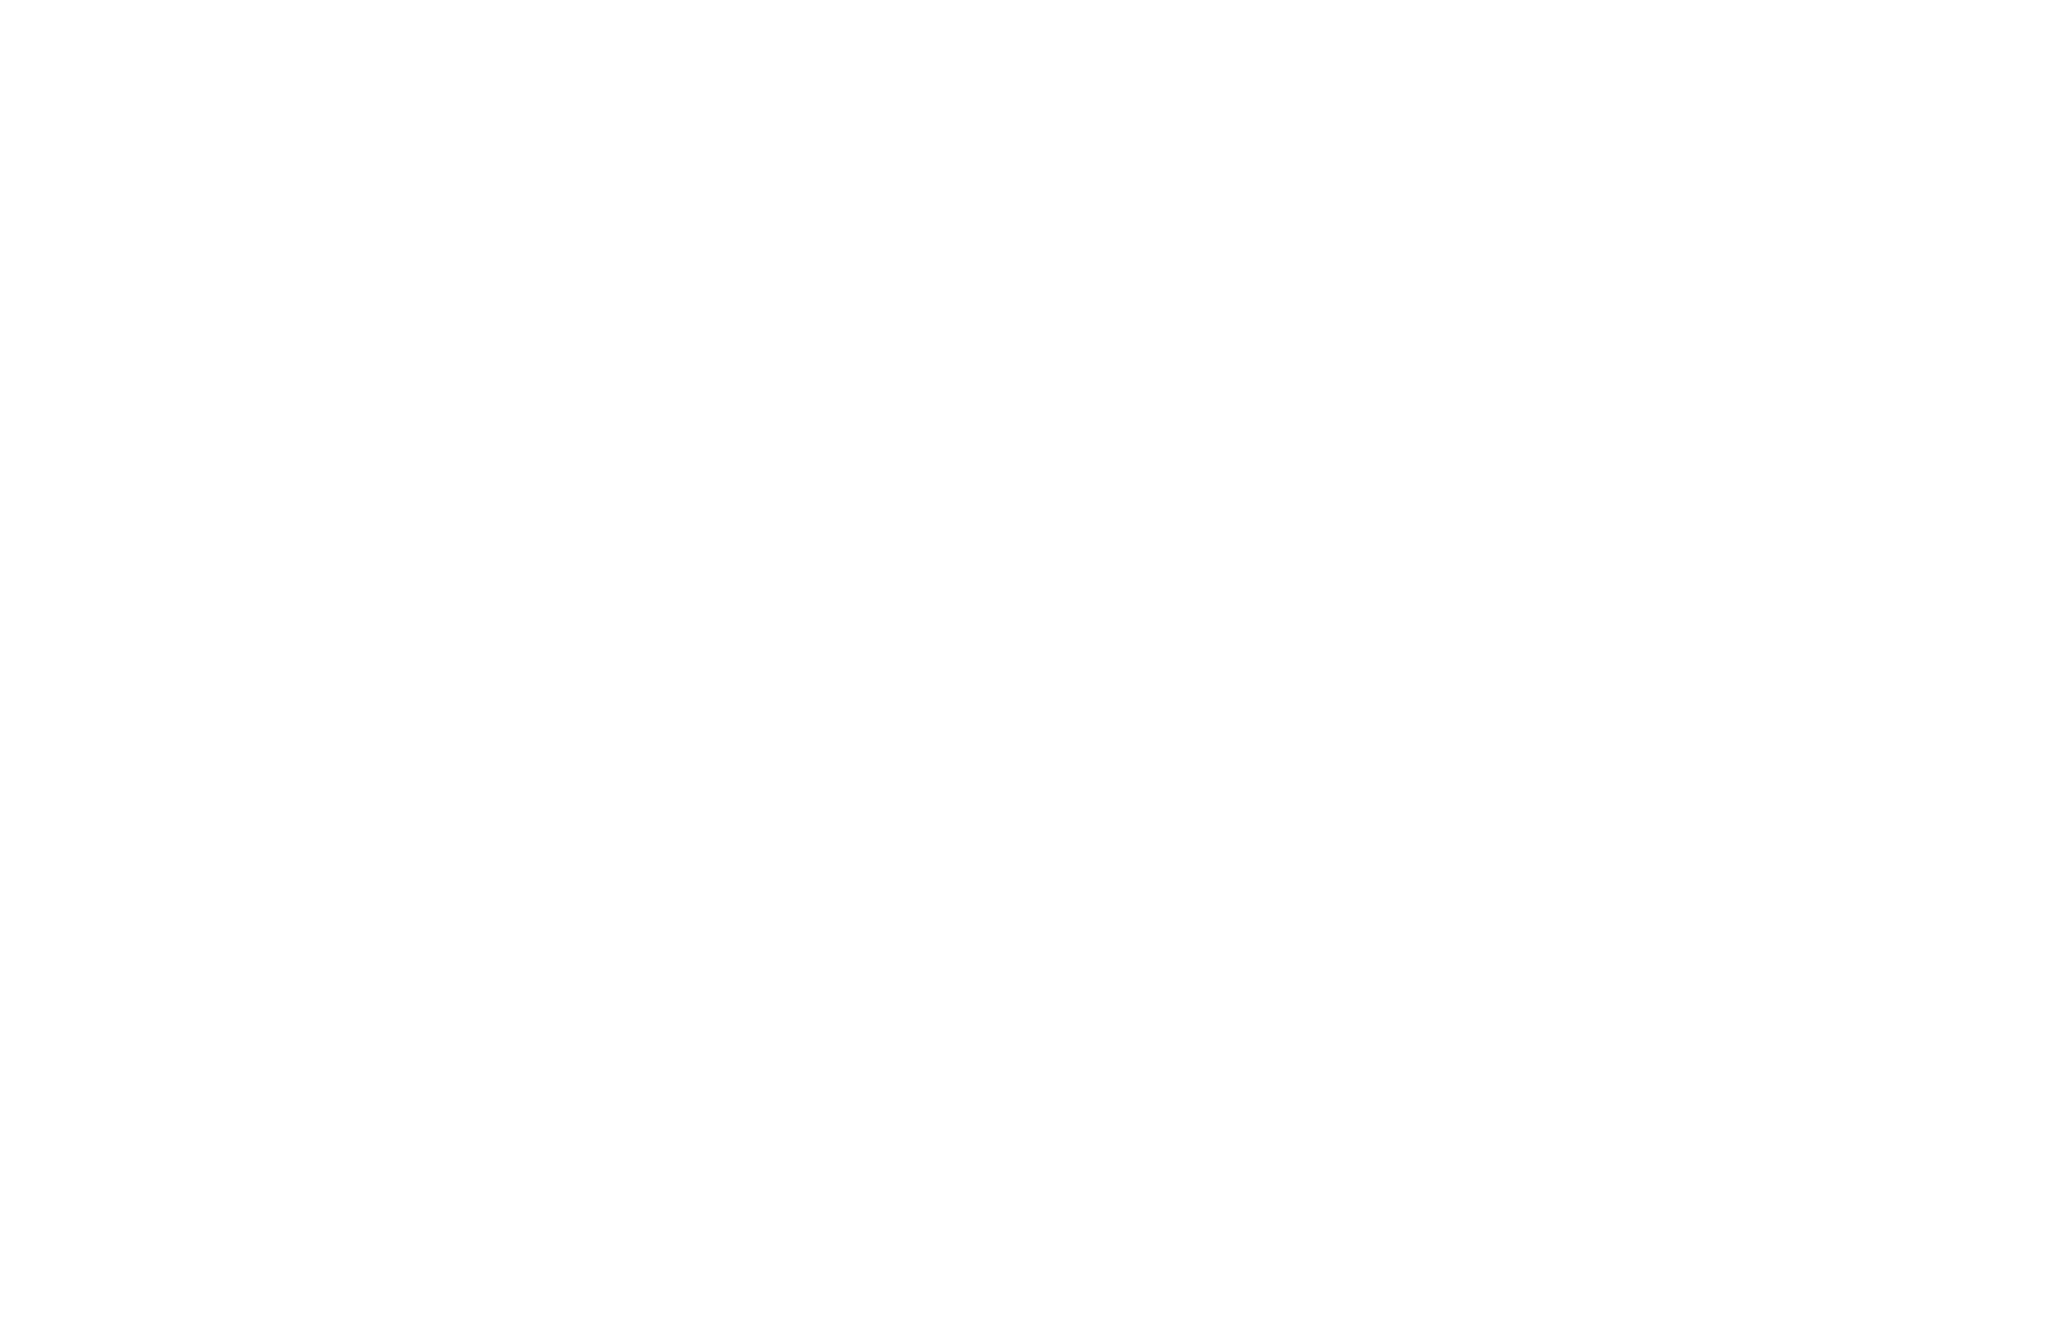
\includegraphics[width=0.9\columnwidth]{images/etl_process.pdf}
  \caption[ETL process within a company]{\gls{ETL} process within a company \citep[pg. 165]{wood2014linked}}
\label{fig:images_etl_process}
\end{figure}

Although this description basically resembles the required activities as explained in the conceptual overview of the \gls{E-commerce} fraud investigation system before, these \gls{ETL} processes generally rely on an in-depth knowledge of the data structures that are used in each of the information sources, as well as require a direct access to the databases and files for retrieving the information. Although these preconditions are not cumbersome to work with \emph{within} an organization, they are not suitable for situations, in which one has to integrate data sources across company boundaries. As the integration of the information takes place on the database level, grant external partners access your internal databases will not only open up access to your business internals, but will also make it much more complicated to change the underlying database structures and business-related software tools. Any changes to one of these would require an elaborate negotiation between the owner of a data source and all of the external partners depending on it. \\

Beside these drawbacks, which make the \gls{ETL} approach unsuitable for the \gls{E-commerce} fraud investigation scenario as a whole, one can assume that these \gls{ETL} processes are still in use for operating the daily business of each stakeholder involved. They can be helpful in the discussion later (see Section~\ref{sec:working_semantic_data}) when a decision has to be made about how each stakeholder can prepare and transform his internal data sources for external consumptions.

% section etl_process

\subsection{Web Services}
\label{subsec:web_services}

With the development of the \gls{E-commerce} scenario there was also a need to integrate business functionalities from various service providers on the Internet. Valid examples for these kind of integrations are the usage of the \gls{PSP}s for doing the payment as well as the \gls{LSP}s for handling the shipping process. These approaches resulted in the ``Service Oriented Architecture'' paradigms, which enable application services provided by different vendors to talk to each other via a public facing programming interface (aka \gls{API}). The only requirement for such interoperability to work properly is that each public interface follows some standardized or commonly agreed upon guidelines to be vendor-, platform- as well as programming language-agnostic. One possible implementation of these concepts are the so-called \emph{Web Services}, which use the WS* protocols and standards from the \gls{W3C} with the extensible markup language (aka \gls{XML}) and the \gls{HTTP} protocol at their core \citep{josuttis2007soa}. \\

Like the \gls{HTML} format, which is used to represent Web pages on the Internet, \gls{XML} is originally based on \gls{SGML}, but instead of formalizing markup tags for structuring and styling textual content it is a meta-language allowing everyone to define their own markup languages. In this matter it doesn’t dictate what tags are available to structure the information; instead it includes some basic guidelines for creating well-formed and valid documents that uses domain-specific tags, which can be freely defined and structured by the creator of the \gls{XML} document. Therefore it is better suited in situations, in which a computer has to parse and evaluate the content of a message; assuming the computer program knows the structure of that message. In an additional step the author of the \gls{API} could also specify an \gls{XML} schema for each message, which describes the structure of the message with all the possible elements, their ordering, nesting level and data types in detail. By doing so the \gls{XML} parser program can later verify the content of a message received against the \gls{XML} schema, and validate if it is a valid document related to that schema definition. \gls{XML} schemata are also expressed in \gls{XML} format and have been standardized by the \gls{W3C}. \\

Being able to create custom markup languages via \gls{XML} has a huge benefit for machine-to-machine communication and is the basis for integrating Web Services (via the WS* protocols), but it still has limitations when it comes to figure out the semantics of those \gls{XML} messages. This is mostly due to the fact that each \gls{XML} document represents a new markup language and needs a specific \gls{XML} parser to be understood by the machine; also to distinguish commonly used tag names in an \gls{XML} document the creator has to place them into specific namespaces (aka \gls{XML} namespaces). But these \gls{XML} namespaces further complicate the automatic processing of \gls{XML} documents and increase the necessity to have custom instances of \gls{XML} parsers for each \gls{XML} document \citep{taylor2008p2p}. \\

An integration of information exchanged via Web Services is therefore handled separately for each Web Service interface. Looking at the payment service integration as \emph{one} possible example, the following steps are necessary to allow a merchant to interact with the Web Service of a \gls{PSP}: \@

\begin{itemize}
  \item the \gls{PSP} has to define and implement an interface (aka \gls{API}) that a merchant can use for exchanging information
  \item the \gls{API} includes a set of request/response messages that hold the data being exchanged, usually specified in \gls{XML} format, as well as a list of operations that the interface supports
  \item the \gls{PSP} has to document each of these messages and operations, incl.\ their intended structures and semantics
  \item the \gls{PSP} has to provide access to the \gls{API} via an \gls{HTTP} endpoint running on a server at a specific \gls{URL}
  \item the \gls{PSP} usually restricts access to this interface for registered partners only; for doing so they have to provide a registration and identification mechanism
  \item the merchant has to register with the \gls{PSP} to be able to call into the Web Service \gls{API}
  \item the merchant receives some kind of token that can be used to identify with the Web Service later
  \item the merchant has to implement an \gls{API}-specific client-side wrapper that knows how to talk to the interface; incl.\ calling one of the available operations as well as serializing and deserializing the messages, which will be transmitted between the Web Service and the client program
  \item the client program from the merchant has to understand the structures and semantics of the messages exchanged with the Web Service and react on them accordingly
\end{itemize}

Although other merchants, who want to use the same \gls{API} from the \gls{PSP}, can use the same client-side wrapper, which is sometimes also provided by that \gls{PSP} for convenience, to be able to send/receive messages to/from this specific Web Service, they still have to make the \gls{API}-specific integrations into their own Web shops. Also these integrations are only done in an one-way direction. To allow the merchants to provide information from their own databases, the merchants have to do likewise and provide an \gls{API} that others can use to query for information by following the same steps as mentioned above. \\

Additionally, as the structures and semantics of the messages and operations of each Web Service interface are not standardized, integrating with \gls{API}s from other \gls{PSP}s or issuers result in doing the same integration steps again and again. To make things worse, the mapping and linking of the information coming from different \gls{API}s have to be implemented by each client to be able to analyze the combined data sets. It becomes clear soon that these necessary tasks will increase the time and efforts with each additional stakeholder, who wants to participate in the collaborative system, see Figure~\ref{fig:web_services_scenario}. \\

\begin{figure}[!ht]
  \centering
  \includegraphics[width=0.9\columnwidth]{images/web-services-scenario.pdf}
  \caption{Data integration within the Web Service approach}
\label{fig:web_services_scenario}
\end{figure}

As conclusion one could say that integrating information between a larger group of participants is very limited with the existing Web Service approach. The steps necessary for exchanging information result in huge efforts on all participating parties. As there is no common way to access and combine the information from each of the participants, beside using the fundamental \gls{HTTP} protocol and \gls{XML} data format, there have to be a lot of collaborative work between each of them upfront to come up with an approach for integrating the available \gls{API}s, and provide the rules for combining the different data structures. Due to these restrictions one can assume that an integration based on the Web Service approach will only work well with a limited number of participants. This might lead to a collaborative system that will only include larger online merchants, \gls{PSP}s and issuers as participants, and therefore left out smaller companies from the \gls{E-commerce} fraud investigation process. For a solution of the problem described in Section~\ref{sec:scope_thesis} this is not sufficient. Due to this limitations one will need other technologies that provide a better scalability and integration ability for the exchange of information between various, otherwise not strongly related organizations.

% subsection web_services (end)

\subsection{Semantic Web}
\label{subsec:web_data}

``The Web is full of intelligent applications, with new innovations coming every day'' \citep{allemang2011semantic}. But each of these intelligent Web applications are \emph{solely} driven by the data available to them. Information that are likely coming from different places in the global information space, accessible usually via a custom \gls{API} on a server hosting those resources (see Section~\ref{subsec:web_services}). The more consistent the information available to the smart Web application are, the better the service and its result will be. But to support an integration of the data from various Web services the semantics of the information delivered by each of them have to be available, and there has to be a generalized, formalized way to express the semantic of that data. The focus on a standard that enables Web services to express the semantics of the data, also allows for global scalability, openness and decentralization, which are the key principles of the World-Wide Web. The \emph{Semantic Web} tries to give a solution for this problem by providing the Resource Description Framework (aka \gls{RDF}) and related technologies (e.g. RDF schema, \gls{SPARQL}, \ldots) for describing, linking and querying the data that a Web service delivers. But it doesn’t reinvent the wheel; instead the Semantic Web builds upon existing, proven technologies such as \gls{XML}, \gls{XML} namespaces, \gls{XML} schemata, and the \gls{URI} to uniquely address resources on the Web \citep{allemang2011semantic}. \\

The main benefits of the Semantic Web approach are the specification of a standardized and generalized format to exchange information on the Web (aka \gls{RDF}) as well as a commonly agreed way to access and query for them (aka \gls{SPARQL}). The \gls{RDF} data format does not only specify the syntax of the information exchanged, but also include the semantics (aka meanings) of them. Due to this fact resources described in \gls{RDF} format are consistent and semantically self-contained. These characteristics are achieved by providing information as a ``triple''; that is a statement consisting of the resource in question (aka subject), a predicate and the specific value (aka object) for it. To be able to unambiguously identify the meaning of these statements, each part of such a ``triple'' is usually expressed with a unique \gls{URI}. These \gls{URI}s can be abbreviated via ``prefix'' definitions to make the whole statement easier to read (see also Section~\ref{sec:semantic_web}). To specify that there is an order ``12345'' from a ``merchant1'', one can come up with the following \gls{RDF} statement, which uses the Schema.org \gls{RDF} vocabulary \citep{Schema.org} to describe an order: \@

\begin{listing}[H]
  \inputminted[linenos,
               numbersep=5pt,
               breaklines=true,
               frame=lines]{TURTLE}
               {./samples/sample_order_12345.ttl}
  \caption{An order specification in \gls{RDF}}
\label{lst:sample_order_ttl}
\end{listing}

An \gls{RDF} file can contain one or more of such ``triples'' describing the resources of interest in detail. Usually these ``triples'' are visualized as directed graph, in that subjects and objects are displayed as nodes and their predicates as edges between them. The order resource shown in the Listing~\ref{lst:sample_order_ttl} above can also be visualized as graph as shown in Figure~\ref{fig:sample_order_graph_image}. \@

\begin{figure}[H]
  \centering
  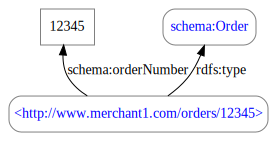
\includegraphics[width=0.8\columnwidth]{images/sample_order_12345.pdf}
  \caption{Graph-based visualization of the order from Listing~\ref{lst:sample_order_ttl}}
\label{fig:sample_order_graph_image}
\end{figure}

Additionally, the \gls{RDF} format has build-in support for merging information from different data sources. This functionality is only working as expected if the ``triples'' in the dispersed data stores are using the same \gls{URI}s to refer to the same subjects or objects. In that situation merging the ``triples'' from different \gls{RDF} data sets will result in a locally linked data set holding the combined information as shown in Figure~\ref{fig:images_combine_rdf_graph}. \@

\begin{figure}[H]
	\centering
		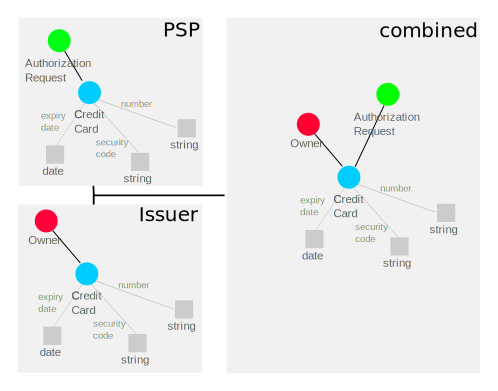
\includegraphics[width=0.9\columnwidth]{images/combine_rdf_graph.pdf}
	\caption{Combining two \gls{RDF} files containing the same credit card entity}
\label{fig:images_combine_rdf_graph}
\end{figure}

Beside being able to provide internal resources in an understandable \gls{RDF} format for external consumption, the Semantic Web also specifies how to query and access these ``information databases'' on the Web. For that purpose the \gls{SPARQL} protocol and query language has been defined. It does not only describes a language to query for information located in \gls{RDF} data stores, but also specifies how to setup an \gls{HTTP} endpoint on a server to make the \gls{RDF} data set publicly available on the Internet. \\

Following the specifications of the Semantic Web standards each relevant participant of an \gls{E-commerce} fraud investigation system will have to transform the information from their internal databases into a set of ``triples'' with commonly agreed upon \gls{URI} references and persist them into a \gls{RDF} data store. For this transformation process an extension of the existing \gls{ETL} processes in an organization can be used. Additionally, these \gls{RDF} data sets will be made available publicly on the Web for information retrieval via the \gls{SPARQL} protocol and query language. Each participant of the collaborative system will only need to know the specific addresses of these \gls{HTTP} endpoints to be able to query them for information. The results of each query can be easily combined into the local \gls{RDF} data set based on the merging capabilities of the \gls{RDF} standard. This will decrease the efforts for integrating the data from various external sources drastically. Also communicating with the different \gls{HTTP} endpoints to access and query for information is being done in a much more efficient way based on the \gls{SPARQL} protocol and query language, see Figure~\ref{fig:web_data_scenario}. \@

\begin{figure}[H]
  \centering
  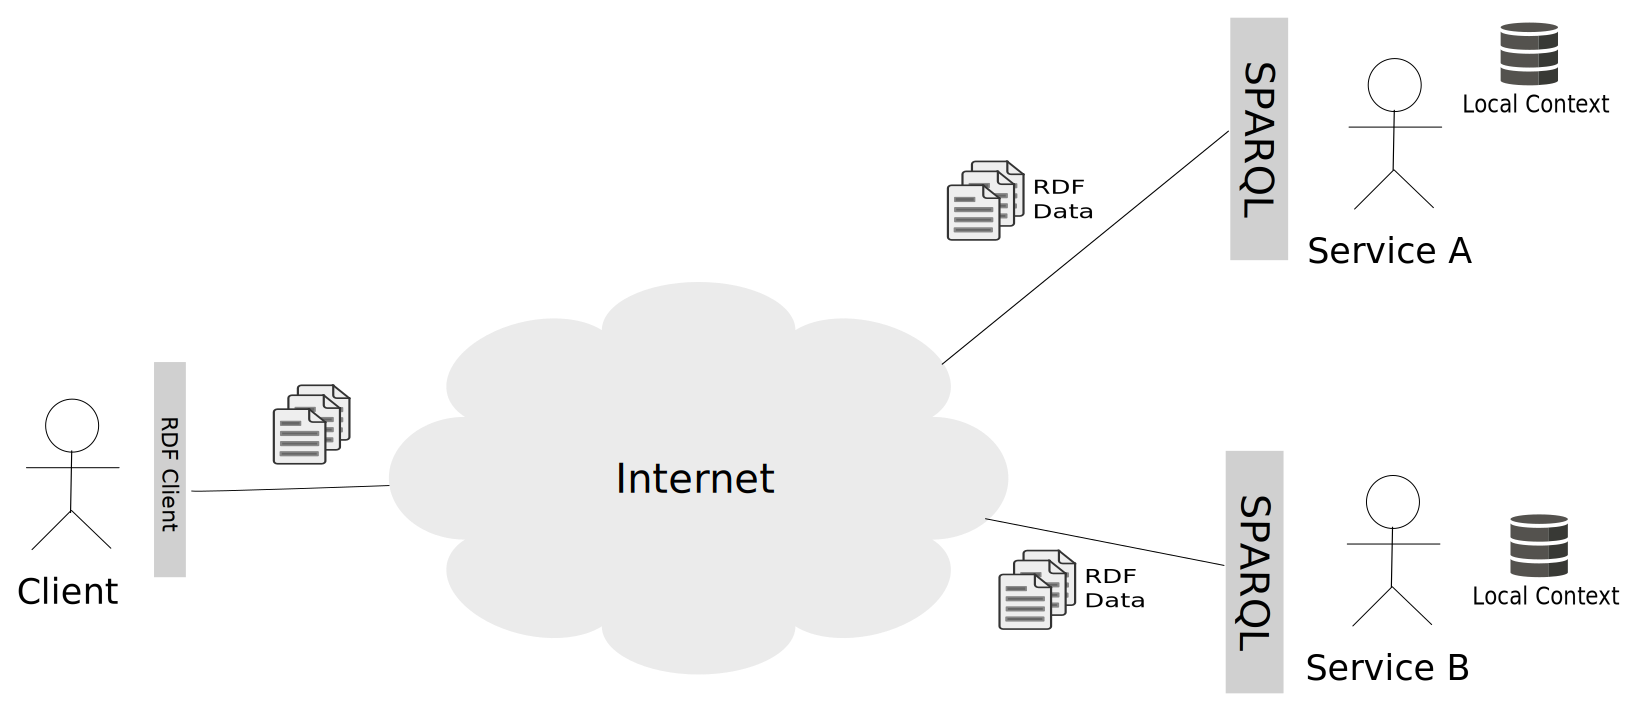
\includegraphics[width=0.9\columnwidth]{images/web-data-scenario.pdf}
  \caption{Data integration within the Semantic Web approach}
\label{fig:web_data_scenario}
\end{figure}

As the underlying model of a \gls{RDF} data set is resembling a graph-based data model it will fit the concept of the proposed system from Section~\ref{sec:analyze_transactions} perfectly. Still requiring every participant to setup and operate a public available \gls{SPARQL} server will limit the use of this approach for the solution of the \gls{E-commerce} fraud investigation scenario. As parts of the information that have to be exchanged between the relevant participants are confidential and/or business-critical, requiring a public \gls{SPARQL} endpoint on the Internet is a high security risk. Additionally the \gls{SPARQL} protocol and query language does not offer a way to restrict access to only a subset of the information in the \gls{RDF} data stores. Any party, who is aware of the \gls{URL} of a \gls{SPARQL} endpoint, have access to all the information that are in the underlying \gls{RDF} data stores and can easily retrieve them with a single \gls{SPARQL} query (see Listing~\ref{lst:get_them_all_sparql}). It is therefore no surprise that there are only a small set of publicly available \gls{SPARQL} endpoints on the Internet --- with the most commonly used one from DBpedia.org \citep{dbPedia.org}, which offers publicly available information from Wikipedia articles in \gls{RDF} format. \@

\begin{listing}[H]
  \inputminted[linenos,
               numbersep=5pt,
               breaklines=true,
               frame=lines]{SPARQL}
               {./samples/get_all_records.sparql}
  \caption{Retrieving all information in an \gls{RDF} store using \gls{SPARQL}}
\label{lst:get_them_all_sparql}
\end{listing}

To conclude, one can assert that the fundamental technologies of the Semantic Web standards are a good fit for exchanging and merging information between different stakeholders. But the usage of an all or nothing approach for querying the \gls{RDF} data stores via the \gls{SPARQL} protocol and query language is way to open for the \gls{E-commerce} fraud investigation system.

% subsection web_data (end)

% section system_approaches (end)
